\documentclass[fr]{../../../../../../epltest}
\usepackage{graphicx}
\usepackage{float}

\hypertitle{Chimie FSAB1301}{2}{FSAB}{1301}{2013}{Mars}{All}
{Martin Braquet }
{Sophie Demoustier, Alain Jonas et Bernard Nysten}

		\section{}
    
    Une marmite en cuivre de 2 kg (couvercle y compris) est portée à $150^{\circ}$C. Rapidement, on verse 100 g d'eau à $25^{\circ}$C et on remet le couvercle. La vapeur d'eau ne s'échappe pas et l'ensemble n'échange pas de chaleur avec l'environnement. Déterminez la température finale du système (marmite plus eau) à l'équilibre.
    
    Quel sera la quantité d'eau liquide transformée en vapeur d'eau?
    
    \textbf{Données:}
    \begin{itemize}
        \item Chaleur spécifique du cuivre = $0,39 J/(g.K)$
        \item Chaleur spécifique de l'eau = $4,18 J/(g.K)$
        \item Enthalpie de vaporisation de l'eau = $40,63 kJ/mol$
    \end{itemize}
    
    \begin{solution}
    
    Supposons que l'eau ne reçoive pas assez de chaleur pour s'évaporer. La température serait alors inférieure à $100^{\circ}$C.
    $$E_{chauff,H_2O}+E_{refroid,Cu}=0$$
    $$100*4,18*(T-298)+0,39*2000*(T-423)=0$$
    $$\Rightarrow T=106,4 ^{\circ}C$$
    Puisque la température est supérieure à $100^{\circ}$C, ce résultat est erroné, une certaine quantité d'eau se présente sous forme de vapeur.
    
    Le liquide sera donc à $100^{\circ}$C, l'énergie supplémentaire fournie par le refroidissement du cuivre servira à transformer un certaine quantité d'eau liquide à à $100^{\circ}$C en phase gazeuse.
    $$E_{chauff,H_2O}+E_{refroid,Cu}+x*\Delta_vap H_{H_2O}=0$$
    avec $x$ le nombre de moles d'$H2O$ sous forme vapeur.
    $$100*4,18*(373-298)+0,39*2000*(373-423)+40630x=0$$
    $$\Rightarrow x=0,1883 \; mol\Rightarrow m_{H_2O(g)}=x*M_m=18x=3,389\:g$$
		
    \end{solution}
    
    \section{}
    
    100 g d'un minerai contenant un mélange d'oxydes de cobalt, $CoO$ et $Co_2O_3$ ainsi que du carbonate de sodium $CaCO_3$ sont traités à l'aide de monoxyde de carbone, $CO$. Les fumées libérées contiennent uniquement 75 g de dioxyde carbone, $CO_2$. Après réaction, on obtient d'une part un métal impur constitué de 90\% molaire de cobalt et 10\% molaire de $Co_2O_3$ et d'autre part 10 g d'une scorie comportant comme seul composé, l'oxyde de cobalt tricalcique $3CaO-Co_2O_3$.
    \begin{enumerate}
        \item Déterminez la quantité en grammes de cobalt présente dans le métal impur.
        \item Donnez la configuration électronique du cation de l'oxyde $Co_2O_3$.
        \item Combien d'électrons non-appariés possède chacun des ions $CoO$?
        \item Donnez un atome isoélectronique du cation de $CoO$.
        \item Classez pas ordre d'électroaffinité croissante les ions des deux oxydes $CoO$ et $Co_2O_3$.
    \end{enumerate}
    
		\begin{solution}
    
    \begin{enumerate}
        \item
    Voici les compositions initiale et finale du mélange:
    \begin{description}
        \item[Initiale]
        \begin{itemize}
            \item 100 g de mélange ($CoO$, $Co_2O_3$ , $CaCO_3$)
            \item $CO$ ($m_{CO}$)
        \end{itemize}
        \item[Finale]
        \begin{itemize}
            \item 75 g de $CO_2$
            \item Métal impur ($m_{MI}$): $Co_2O_3$(0,1\%) et $Co$ (0,9\%)
            \item 10 g de scorie: ($3CaO-Co_2O_3$)
        \end{itemize}
    \end{description}
    
     La fraction massique de $C$ dans la scorie est
     $$3\frac{M_{m,C}}{M_{m,scorie}}=3*16/323=0,14815$$
      La fraction massique de $C$ dans le $CO_2$ est
     $$\frac{M_{m,C}}{M_{m,CO_2}}=16/44=0,36364$$
     La fraction massique de $C$ dans le $CO$ est
     $$\frac{M_{m,C}}{M_{m,CO}}=16/28=0,5714$$
     Par conservation du nombre de moles de $C$, on calcule $m_{CO}$
     $$0,5714m_{CO}=0,36364m_{CO_2}+0,14815m_{scorie}$$
     $$\Rightarrow m_{CO}=50,32g$$
    Par conservation de la masse totale,
    $$100g+50,32g=75g+10g+m_{MI}$$
    $$\Rightarrow m_{MI}=65,32g$$
    Cela mène à un système:
    $$M_{m,Co_2O_3}\:n_{Co_2O_3}+M_{m,Co}\:n_{Co}=65,32$$
    et
    $$n_{Co}=9\:n_{Co_2O_3}$$
    $$\Rightarrow n_{Co}=0,8434\:mol \Rightarrow m_{Co}=49,76g$$
    
    \item Le cation est $Co^{3+}$, il a 24 $e^-$ (Z-3). Sa configuration électronique est une exception:
    $$1s^2\: 2s^2\: 2p^6\: 3s^2\: 3p^6\: 3d^6$$
    
    \item Les ions sont $Co^{2+}$ et $O^{2-}$, il y a donc 2 électrons non appariés pour chaque ion.
    
    \item Un atome possédant le même nombre d'électrons que $Co^{2+}$ (isoélectronique) est le $Mn$ puisqu'il a 25 électrons.
    
    \item $$O^{2-}<Co^{2+}<Co^{3+}$$
        Les ions possédant un déficit d'électrons (cations) ont une électroaffinité élevée. 
    
    \end{enumerate}
    
		\end{solution}
		
    \section{}
    
    L'acide fumarique (E297) est un acide dicarboxylique (porteur de deux fonctions acides) insaturé naturel présent dans la plupart des fruits et dans de nombreux légumes dont la formule est $(CH)_2(COOH)_2$. Afin de titrer (déterminer la concentration) une solution inconnue d'acide fumarique, on dilue celle-ci 10 fois. Par ailleurs, on dissout 5 g de soude ($NaOH$) dans 500 mL d'eau distillée. Afin de neutraliser complètement 100 mL de solution diluée d'acide, il faut ajouter 30 mL de solution de soude. Quelle est la concentration en g/L de la solution initiale (non diluée) d'acide fumarique?
    
    \begin{solution}    
    
    La réaction s'écrit:
    $$(CH)_2(COOH)_2+2NaOH\Rightarrow (CH)_2(COONa)_2+2H_2O$$
    On constate qu'une mole de $(CH)_2(COOH)_2$ réagit avec 2 moles de $NaOH$.
    
    Soit x, la concentration initiale non diluée de la solution de $(CH)_2(COOH)_2$.
    Le nombre de moles réagissant dans cette solution (de 100 mL) est 
    $$0,1xV_{(CH)_2(COOH)_2}/M_{m,(CH)_2(COOH)_2}=x\frac{0,1*0,1}{116}=x/11600\:mol$$
    et le nombre de moles de $NaOH$ est 
    $$C_{NaOH}V_{NaOH}/M_{m,NaOH}=\frac{10*0,03}{40}=7,5*10^{-3}\:mol$$.
    On obtient donc
    $$2n_{(CH)_2(COOH)_2}=n_{NaOH}\Rightarrow x=7,5*10^{-3}*11600/2=43,5\:g/L$$
    
		\end{solution}
		
    \section{}
		
    \begin{enumerate}
        \item Donnez la structure de Lewis de l'acide fumarique.
        \item Tous les atomes de cette molécule peuvent-ils se trouver dans le même plan? Justifiez votre réponse.
        \item La notion d'hybridation est-elle nécessaire pour expliquer la formation et l'orientation des liaisons dans cette molécule? Si oui, donnez l'hybridation des 4 atomes de carbone et des 4 atomes d'oxygène.
        \item Expliquez comment se sont formées les liaisons carbone-oxygène.
    \end{enumerate}
    
    \begin{solution}
		
    \begin{enumerate}
    
        \item 
        
           \begin{figure}[H]
            \centering
            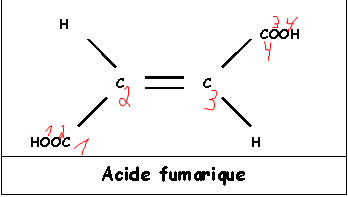
\includegraphics[scale=0.5]{AcFum}
            \end{figure}
						
        \item 
        Les atomes ne sont pas dans le même plan. Les 2 atomes $O$ liés chacun à un $H$ sont hybridés $sp^3$ et ont donc une configuration tétraèdrique. Ils ont une liaison simple avec un O, une autre liaison simple avec un H et 2 doublets non liants. Le H n'est donc pas dans le même plan que le reste de la molécule.
        \item 
        La notion d'hybridation est bien nécessaire. 
        \begin{itemize}
            \item $O_1$ et $O_4$ sont hybridés $sp^3$
            \item $O_2$ et $O_3$ sont hybridés $sp^2$
            \item Les 4 $C$ sont hybridés $sp^2$
        \end{itemize}
        \item 
        \begin{itemize}
            \item Liaison entre $C_1$ et $O_1$: (liaison double) liaison $\sigma$ par recouvrement axial et liaison $\pi$ par recouvrement latéral d'orbital
            \item Liaison entre $C_1$ et $O_2$: (liaison simple) liaison $\sigma$ par recouvrement axial 
        \end{itemize}
    \end{enumerate}
    
\end{solution}

\end{document}
